\documentclass{article}
\usepackage{pgfgantt}
\usepackage{float}
\title{Timeline for pre-submission}
\date{}
\pagenumbering{gobble}
\begin{document}

\maketitle

\vspace{-1.5cm}

I have already completed a first draft of chapter 3 and have completed the majority of the chapter 4 already. Chapter 5 is already begun, and in general will be more descriptive of analysis that has already been finished, rather than an in-depth account of an experiment like chapter 4. 

Chapters 1 and 7 have not been started, which is why they are alloted more time. Chapter 2 is similar, but will be a summary of linear collider projects and can be based on existing information and technical reports, so will be easier (and faster) to produce. 

\vspace{0.5cm}

\begin{figure}[H]
\centering
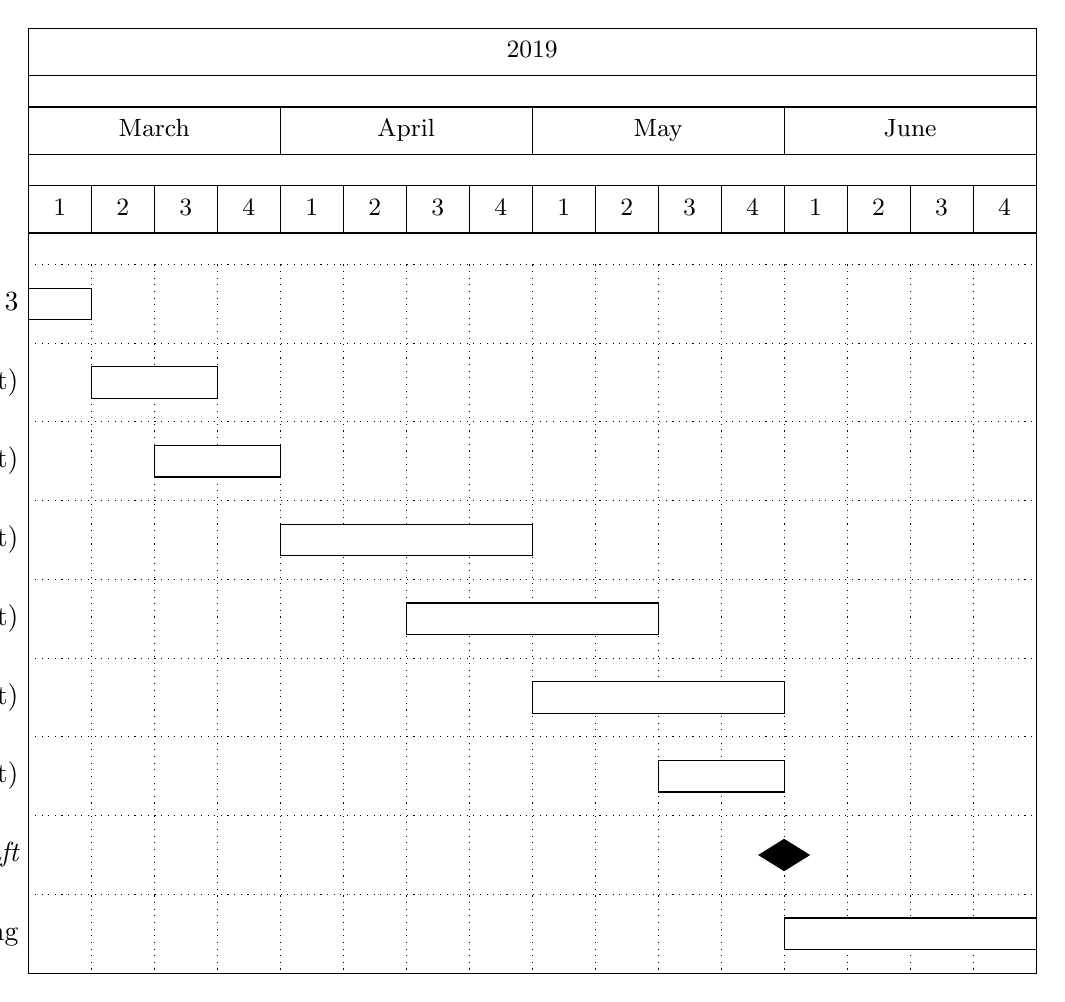
\begin{tikzpicture}
\begin{pgfinterruptboundingbox}
\begin{ganttchart}[canvas/.append style={alias=frame},hgrid,vgrid,x unit=0.8cm]{1}{16}
  \gantttitle{2019}{16} \\
  \gantttitlelist{"March","April","May","June"}{4} \\
  \gantttitlelist{1,2,3,4,1,2,3,4,1,2,3,4,1,2,3,4}{1} \\
  
  \ganttbar{Chapter 3}{1}{1} \\
  
  \ganttbar{Chapter 4 (1\textsuperscript{st} draft)}{2}{3} \\

  \ganttbar{Chapter 5 (1\textsuperscript{st} draft)}{3}{4} \\
  
  \ganttbar{Chapter 6 (1\textsuperscript{st} draft)}{5}{8} \\
  \ganttbar{Chapter 7 (1\textsuperscript{st} draft)}{7}{10} \\
 
  \ganttbar{Chapter 1 (1\textsuperscript{st} draft)}{9}{12} \\
  \ganttbar{Chapter 2 (1\textsuperscript{st} draft)}{11}{12} \\
  
  \ganttmilestone{Completed first draft}{12} \\

  \ganttbar{Editing and finalising}{13}{16}
\end{ganttchart}
\end{pgfinterruptboundingbox}
\useasboundingbox (frame.south west) rectangle (frame.north east);
\end{tikzpicture}
\end{figure}



\end{document}